\documentclass{book}\usepackage{knitr}

% Preamble

%%%%%%%%%%%%%%%%%%%%%%
%% PACKAGES
%%%%%%%%%%%%%%%%%%%%%%
\usepackage[twoside,letterpaper,width=6in,height=8in]{geometry}
\usepackage{siunitx} % format units properly
\usepackage{wrapfig}
\usepackage[margin=10pt,font=small,labelfont=bf]{caption} % format captions
\usepackage{booktabs} % nicer tables
\usepackage{subcaption} 
\usepackage{csquotes} % block quotes
\usepackage{tikz}
\usepackage[inline, shortlabels]{enumitem} % inline enumeration
%\usepackage[version=4]{mhchem}
\usepackage{graphicx} % packages are used to modify the text and create bling.
%\includegraphics{{Home/CAMPUS/mwl04747/github/Environmnental-Sciences-in-East-Asia/images/}}
\usepackage{textcomp}
\usepackage{gensymb}
\usepackage{natbib}
\usepackage{glossaries}
\usepackage{amsmath}%
\usepackage{amsfonts}%
\usepackage{amssymb}%

%\usepackage[super,square,comma]{natbib}
%\usepackage{float}
%\usepackage{appendix}
%\usepackage{chngcntr}
%\usepackage{etoolbox}
%\usepackage[usenames]{xcolor}% for commenting in color!

\RequirePackage{hyperref} % For hyperlinked cross-references
\hypersetup{
    colorlinks,
    citecolor=blue,
    filecolor=blue,
    linkcolor=blue,
    urlcolor=blue
}


%----------------------------------------------------------
\newtheorem{theorem}{Theorem}
\newtheorem{acknowledgement}[theorem]{Acknowledgement}
\newtheorem{definition}[theorem]{Definition}
\newtheorem{example}[theorem]{Example}
\newtheorem{exercise}[theorem]{Exercise}

\newtheorem{problem}[theorem]{Problem}
\newtheorem{remark}[theorem]{Remark}
\newtheorem{solution}[theorem]{Solution}
\newtheorem{summary}[theorem]{Summary}
\newenvironment{proof}[1][Proof]{\textbf{#1.} }{\ \rule{0.5em}{0.5em}}
%----------------------------------------------------------

\AtBeginEnvironment{subappendices}{%
\chapter*{Appendix}
\addcontentsline{toc}{chapter}{Appendices}
%\counterwithin{figure}{section}
%\counterwithin{table}{section}
}

\makeatletter
\newcommand{\chapterauthor}[1]{%
  {\parindent0pt\vspace*{-25pt}%
  \linespread{1.1}\large\scshape#1%
  \par\nobreak\vspace*{35pt}}
  \@afterheading%
}
\makeatother

\renewcommand{\glstextformat}[1]{\textbf{\color{blue}\em #1}}

\newcommand{\R}{\mathbb{R}}
\newcommand{\carbondioxide}{CO$_2$~}



\title{Environmental Issues in East Asia}
\author{EA30e Spring 2021}
\date{\today}
\IfFileExists{upquote.sty}{\usepackage{upquote}}{}
\begin{document}

\maketitle
\makeglossaries

\frontmatter
\tableofcontents


\chapter*{Preface}

\section{Guiding Principles}

Environmental issues in East Asia are not unique or particularly more prevasive than other parts of the world. However, the issues are born from particular histories that may contrast with other parts of the world and other parts of the world may be able to learn from. 

In this project, the students in EA030e (Spring 2021) have written a textbook that highlights examples of environmental processes. Each student contributed to one theme, composed of two examples that highlight environmental issues of East Asia. 

\subsection{Context and Positionality}

As students in a college course located in Southern California, we approach the project with...


Our goal is not to call out environmental issues in East Asia, but to point to linkages of how a range of globalized economy contribute to these environmental problems. 

In the end, it would be useful for us to acknowledge we have some capacity to address these how these global linkages could be modified to reduce these environmental issues.

We are not experts, but learning... if there are errors please let us know... We recommend that suggestions be submitted via a github pull request.

\subsection{Goals}

Processes across horizontal boundaries define many environmental patterns that frame human interactions with the environment. How do humans impact processes that cross these boundaries and how do humans influence these ecosystem interface?

\subsection{Rationale}

We hope to learn more about the how environmental issues are expressed in different parts of the world and to what extent can we learn from this work. 

\subsection{Activity}

Each group will be composed of two students, that will become experts and teach their classmates on the topic. 

\section{East Asia and the World}







\section{Acknowledgments}

Everyone in the world!




\chapter{Author Guide}\label{ch:guide}

\subsection*{Why Learn \LaTeX?}

In the past, I used \LaTeX to make publication quality text. In fact, many prefer writing in \LaTeX because they can focus on the text and avoid worrying about formatting. However, it is NOT WYSIWYG (``what you see is what you get'') word processor. In reality, the processing or compiling is a separate step. 

Nevertheless, the quality of the output and ability to integrate with R (or Python) allows us to have an exceptional tool to make reproducible documents. 

\subsection*{How to Learn \LaTeX?}

There are several ways to learn \LaTeX. I suggest you find a decent tutorial to get the basics. For example, here are some suggestions:

\begin{itemize}
  \item \href{https://www.overleaf.com/learn/latex/Learn_LaTeX_in_30_minutes}{Learning \LaTeX in 30 minutes}
\end{itemize}

If you are like me and can't remember commands very well, then here's a \href{https://wch.github.io/latexsheet/latexsheet-0.png}{cheet sheet} that might be helpful. 

\subsubsection{R Chunks}

To create effective graphics, each chapter will have a rchunk that creates a graphic for the chapter. To review and learn R, here are some resources: 

\begin{itemize}
  \item \href{www.tbd.com}{Marc's Video Description}
  \item \href{https://rmd4sci.njtierney.com/}{RMarkdown for Scientists (super helpful!)}
  \item \href{https://rmarkdown.rstudio.com/lesson-1.html}{R Studio Tutorial}
  \item \href{https://rstudio.com/wp-content/uploads/2016/03/rmarkdown-cheatsheet-2.0.pdf?_ga=2.107420162.161662097.1613074083-214354297.1613074083}{R Studio's Cheatsheet}
  \item \href{https://bookdown.org/yihui/rmarkdown-cookbook}{R Markdown Cookbook -- Robust Source}
\end{itemize}


\subsection*{Noting Your Contribution}

Because this is an ongoing project, you should record your contribution to each chapter -- but also let go of these contributions at some point; Others might revise and their authorship might take some precedence, so you should both invest in the product but also be willing to detach from the final outcome as others contribute. This will feel uncomfortable at times, but please note from the beginning this is a social process and as such subject to negotiation. Please be generous to the authors that laid the foundation and be respectful of those that follow. 

\section{Setting Up Book Project--Type Setting w/ \LaTeX}

\subsection*{Latex Book Class}

Currently, the text is written using the standard book class. %However, in 2019, I (Los Huertos) will convert the format to a Tufte book class. 

\subsection*{Structuring the Text with Nested Hierarchies}

Contributors divide their contributions into sections and subsections. This format allows a consistent approach to structuring the text and forcing themes to be organized in blocks that can be used to organize the overall text. We use section, subsection, and subsubsection to break up the topic into bite sizes. 

To accomplish this, contributors use the \verb"\section{Section}" command for major sections, and the \verb"\subsection{Subsection}" command for subsections, and a similar approach for subsubsections. 

NOTE: for each nested level, it MUST be followed by the lowest level in the section before a paragraph is started -- in contrast to what is shown above!

NOTE: We may dispense with subsubsections in the future to provide a less blocky structure, but for now they remain useful. 

\subsection*{Font Changes}

We can use various methods to alter the typeset: \emph{Emphasize}, \textbf{Bold}, \textit{Italics}, and \textsl{Slanted}. We can also typeset \textrm{Roman}, \textsf{Sans Serif}, \textsc{Small Caps}, and \texttt{Typewriter} texts.  Look online to see the commands to accomplish these changes. 

You can also apply the special, mathematics only commands $\mathbb{BLACKBOARD}$, $\mathbb{BOLD}$, $\mathcal{CALLIGRAPHIC}$, and $\mathfrak{fraktur}$. Note that blackboard bold and calligraphic are correct only when applied to uppercase letters A through Z.

You can apply the size tags -- Format menu, Font size submenu -- {\tiny tiny}, {\scriptsize scriptsize}, {\footnotesize footnotesize}, {\small small}, {\normalsize normalsize}, {\large large}, {\Large Large}, {\LARGE LARGE}, {\huge huge} and {\Huge Huge}.

You can use the \verb"\begin{quote} etc. \end{quote}" environment for typesetting short quotations. Select the text then click on Insert, Quotations, Short Quotations:

\begin{quote}
The buck stops here. \emph{Harry Truman}

Ask not what your country can do for you; ask what you can do for your
country. \emph{John F Kennedy}

I am not a crook. \emph{Richard Nixon}

I did not have sexual relations with that woman, Miss Lewinsky. \emph{Bill Clinton}
\end{quote}

The Quotation environment is used for quotations of more than one paragraph. Following is the beginning of description of \LaTeX from \emph{Wikipedia}:

\begin{quotation}
LaTeX (/ˈlɑːtɛx/ LAH-tekh or /ˈleɪtɛx/ LAY-tekh, often stylized as \LaTeX) is a software system for document preparation. When writing, the writer uses plain text as opposed to the formatted text found in ``What You See Is What You Get'' word processors like Microsoft Word, LibreOffice Writer and Apple Pages. The writer uses markup tagging conventions to define the general structure of a document (such as article, book, and letter), to stylise text throughout a document (such as bold and italics), and to add citations and cross-references. A \TeX distribution such as \TeX Live or MiK\TeX is used to produce an output file (such as PDF or DVI) suitable for printing or digital distribution.

LaTeX is widely used in academia for the communication and publication of scientific documents in many fields, including mathematics, statistics, computer science, engineering, physics, economics, linguistics, quantitative psychology, philosophy, and political science. It also has a prominent role in the preparation and publication of books and articles that contain complex multilingual materials, such as Sanskrit and Greek. \LaTeX uses the TeX typesetting program for formatting its output, and is itself written in the TeX macro language.''
\end{quotation}

Use the Verbatim environment if you want \LaTeX\ to preserve spacing, perhaps when
including a fragment from a program such as:
\begin{verbatim}
#include <iostream>         // < > is used for standard libraries.
void main(void)             // ''main'' method always called first.
{
 cout << ''This is a message.'';
                            // Send to output stream.
}
\end{verbatim}
(After selecting the text click on Insert, Code Environments, Code.)


\subsection*{Mathematics and Text}

\subsubsection{Warning: Special Characters}

When you use percent and ampersand symbols, hash tags, and other non-standard ASCII characters, \LaTeX will be very uncooperative. So, do yourself a favor and make sure you understand that these are used for special typesetting functions. To use them you have to ``escape'' and use commands to get them to do what you might usually expect!  \% \# \& \`e \~n `` and '' to show a few that do not reflect the key stroke you might expect. 

\LaTeX doesn't like a range of characters or they reserved for special behavior...

For example, the \# is used for tabs in a table environment. \% is used to make comments, thus stuff behind a \% is ignored. There are lots of others, but these come up the most.

\subsubsection{Creating equations}

One of the most powerful parts of \LaTeX is how it can be used to write complex equations, with all those symbols and Greek letters! This can be done inline $y = mx + b + \epsilon$ for fairly simple equations, or set apart for more complex equations:

\begin{equation}
\int_0^\infty e^{-x^2} dx=\frac{\sqrt{\pi}}{2}
\end{equation}

\subsubsection{Theorems, etc}
\begin{theorem}
(The Currant minimax principle.) Let $T$ be completely continuous selfadjoint operator
in a Hilbert space $H$. Let $n$ be an arbitrary integer and let $u_1,\ldots,u_{n-1}$ be
an arbitrary system of $n-1$ linearly independent elements of $H$. Denote
\begin{equation}
\max_{\substack{v\in H, v\neq
0\\(v,u_1)=0,\ldots,(v,u_n)=0}}\frac{(Tv,v)}{(v,v)}=m(u_1,\ldots, u_{n-1})
\label{eqn10}
\end{equation}
Then the $n$-th eigenvalue of $T$ is equal to the minimum of these maxima, when
minimizing over all linearly independent systems $u_1,\ldots u_{n-1}$ in $H$,
\begin{equation}
\mu_n = \min_{\substack{u_1,\ldots, u_{n-1}\in H}} m(u_1,\ldots, u_{n-1}) \label{eqn20}
\end{equation}
\end{theorem}
The above equations are automatically numbered as equation (\ref{eqn10}) and
(\ref{eqn20}).


\subsection{Lists Environments: Making bulletted, numbered, description lists}

We use special commands to create an itemized list.

You can create numbered, bulleted, and description lists
(Use the Itemization or Enumeration buttons, or click on the Insert menu
then chose an item from the Enumeration submenu):

\begin{enumerate}
\item List item 1

\item List item 2

\begin{enumerate}
\item A list item under a list item.

\item Just another list item under a list item.

\begin{enumerate}
\item Third level list item under a list item.

\begin{enumerate}
\item Fourth and final level of list items allowed.
\end{enumerate}
\end{enumerate}
\end{enumerate}
\end{enumerate}

\begin{itemize}
\item Bullet item 1

\item Bullet item 2

\begin{itemize}
\item Second level bullet item.

\begin{itemize}
\item Third level bullet item.

\begin{itemize}
\item Fourth (and final) level bullet item.
\end{itemize}
\end{itemize}
\end{itemize}
\end{itemize}

\begin{description}
\item[Description List] Each description list item has a term followed by the
description of that term.

\item[Bunyip] Mythical beast of Australian Aboriginal legends.
\end{description}

\subsection{Theorem-Like Environments}

The following theorem-like environments (in alphabetical order) are available
in this style.

%\begin{acknowledgement}
%This is an acknowledgement
%\end{acknowledgement}

\begin{example}
This is an example
\end{example}

\begin{exercise}
This is an exercise
\end{exercise}


%\begin{proof}
%This is the proof of the lemma.
%\end{proof}

%\begin{notation}
%This is notation
%\end{notation}

%\begin{problem}
%This is a problem
%\end{problem}

%\begin{proposition}
%This is a proposition
%\end{proposition}

%\begin{remark}
%This is a remark
%\end{remark}

%\begin{summary}
%This is a summary
%\end{summary}

\begin{theorem}
This is a theorem
\end{theorem}

%\begin{proof}
%[Proof of the Main Theorem]This is the proof.
%\end{proof}

%\subsubsection{``Child'' Rnw Contributions}

%This is a chapter that we can input into the text... you will each create a chapter without the preamble and begin and end document... that can be integrated into a single book! 

\subsection{Peer Review Commenting}

You can put your comments in square brackets and in color for things that need help. \textcolor{red}{[This section is confusing, I am not sure what commenting means.]}

\subsection{Adding Figures, etc}

\subsubsection{Using Rnw Files}

To generate R figures, we use R chunks in and Rnw file, where the text is integreated. When we compile into a PDF, the program converts the files into TeX files and then combineds them into a single pdf. 

For each chapter, we create a ``child'' document and Marc will help you create that text when you begin. 

\subsubsection{Creating a floating figure}

This is my floating figure (Figure \ref{fig:plot}).

\begin{figure}

\caption{My plot's caption is here!}
\label{fig:plot}
\end{figure}

\subsubsection{Using R to Create Effective Figures}

R Markdown can be a very powerful tool to integrate R code, figures and text. Making high quality figures that are both clear and aestically pleasing will be something that we need to think about it. 

\begin{itemize}
  \item Axis Labels -- Labelled with clarity 
  \item Axis Text -- Size, Orientation 
  \item Captions (usually better than titles)
  \item References connecting labels to references
  \item ADA accessible (e.g. color impairment mitigation)
\end{itemize}

For example, here's code to generate a pretty good figure: 



\begin{knitrout}
\definecolor{shadecolor}{rgb}{0.969, 0.969, 0.969}\color{fgcolor}\begin{kframe}


{\ttfamily\noindent\bfseries\color{errorcolor}{\#\# Error in file(file, "{}rt"{}): cannot open the connection}}

{\ttfamily\noindent\bfseries\color{errorcolor}{\#\# Error in createDataPartition(., p = 0.8, list = FALSE): object 'maunaloa' not found}}

{\ttfamily\noindent\bfseries\color{errorcolor}{\#\# Error in eval(expr, envir, enclos): object 'maunaloa' not found}}

{\ttfamily\noindent\bfseries\color{errorcolor}{\#\# Error in eval(expr, envir, enclos): object 'maunaloa' not found}}

{\ttfamily\noindent\bfseries\color{errorcolor}{\#\# Error in eval(expr, envir, enclos): object 'maunaloa' not found}}

{\ttfamily\noindent\bfseries\color{errorcolor}{\#\# Error in is.data.frame(data): object 'maunaloa' not found}}

{\ttfamily\noindent\bfseries\color{errorcolor}{\#\# Error in summary(model): object 'model' not found}}

{\ttfamily\noindent\bfseries\color{errorcolor}{\#\# Error in predict(., test.data): object 'model' not found}}

{\ttfamily\noindent\bfseries\color{errorcolor}{\#\# Error in mean((pred - obs)\textasciicircum{}2, na.rm = na.rm): object 'predictions' not found}}\end{kframe}
\end{knitrout}

In the case of Figure \ref(fig:maunaloa), we can a create a figure that has all of the characteristics listed above, except perhaps ADA. Creating a "alt text" for the figure is something we might want to consider. 

\begin{figure}
\begin{knitrout}
\definecolor{shadecolor}{rgb}{0.969, 0.969, 0.969}\color{fgcolor}\begin{kframe}


{\ttfamily\noindent\bfseries\color{errorcolor}{\#\# Error in ggplot(train.data, aes(decimal.date, average)): object 'train.data' not found}}\end{kframe}
\end{knitrout}
\caption{Carbon Dioxide Concentrations (Mauna Loa, HI). Source: Scripps/NOAA.}
\label{fig:co2-graphic}
\end{figure}

\subsection{Using Boxes}

\fbox{
\begin{minipage}[c]{.9\textwidth}
\subsection{minibox X}

Some text
\end{minipage}
}

\subsection{ Cross-References, Citations, and Glossaries}

\subsubsection{Cross-References}

We can cross-reference sections (e.g. Section~\ref{ch:critical-zone}  or figures (Figure~\ref{fig:maunaloa}) using several methods. I suggest you look at the this Rmd file to see how I did it in these examples.

You can also create links to URLs or hyperlinks, e.g. \url{http://texblog.org}. However, if these addresses change, then the link will break, so I suggest you only link to internal references.

\subsubsection{Bibliography generation}

There will be two steps to cite our sources. First, we need to add the reference to a database, or bib file. This is titled 'References.bib' and is located in the main folder in our respository. When you add information to the bib file, be sure to paste in the reference using a bibTeX format. 

Second, we'll need to place in-line citations, using \verb"\citep{knitr}", which produces \citep{knitr}, by using a key, which is knitr in this case. 

For example, you might write, ``This document was produced in RStudio using the knitr package (\citep{knitr}). Also try \verb"\citet{LosHuertos2017OverviewR}" to create use the author name as the subject: \citet{LosHuertos2017OverviewR} wrote an guide to help students learn R. 

Note: You will see these citations automatically put in alphabetic order in the Bibliography at the end of the PDF. 

%Currently, we are using the ecology.bst, but it has trouble with misc type of references, so I will changing this in 2019. 

\subsubsection{Creating glossary words}
 
\newglossaryentry{peat}{
	name=peat, 
	description={is cool.}
}

\begin{definition}
This is a definition and the word is use in an glossary, e.g. \gls{peat}. \Gls{peat} is when you want to capitalize the defined word without having to re-define a capitalized version, the only downside of case sensitivity in \LaTeX.
\end{definition}


\chapter{Chapter Title}

\chapterauthor{Chapter Author Name}

\footnote{Statement of Contributions-- For example, ``The chapter was first drafted by Marc Los Huertos (2021). The author recieved valuable feedback from X, and Y and Z to improve the chapter. Slater revised the chapter in 2022 with suggestions from Cater.'' Note: I am still working on the formatting for this to improve it.}

\section{Section Heading}% Avoid putting text between section and subsection headings.

\subsection{Subsection Headings} % Avoid putting text between subsection and subsubsection headings. Not applicable if you don't have subsections!

Some text here... if you cut and paste, be sure to make sure you don't include formatted characters outside the ASCII values. See Author Guide\ref{ch:guide}.

\subsubsection{Optional Subsubsection Headings} % Again try to avoid putting text between the subheadig and the subsubheading to main a structural consistency.

some text here....

\section{Goals of this template}

This template will NOT teach you how to use \LaTeX! To accomplish that, we'll rely on some great online resources that you can find on in Chapter \ref{ch:guide}. 

Instead this section of the document is designed to demonstrate how our textbook will look, feel, and ultimately how we contribute to the project.

This document also compiles all of our projects into a single PDF, where each chapter is composed of a input tex file.

\section{Here's figure}

\subsection{R Created Figures}

First we create an R chunk and add some code. In this case, I created a floating figure which can be referenced (Figure~\ref{fig:pressure})!  

\begin{figure}
\begin{knitrout}
\definecolor{shadecolor}{rgb}{0.969, 0.969, 0.969}\color{fgcolor}\begin{kframe}
\begin{alltt}
\hlkwd{plot}\hlstd{(pressure)}
\end{alltt}
\end{kframe}
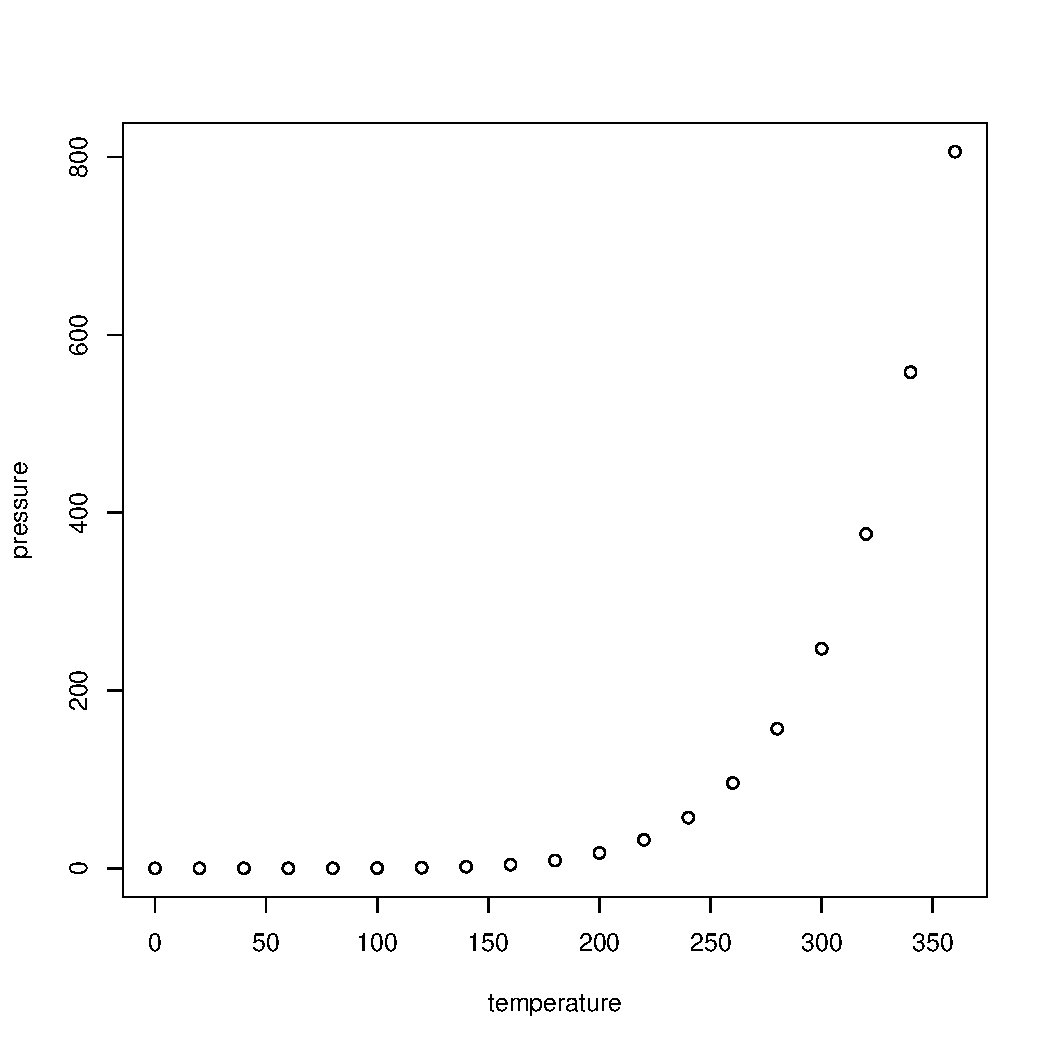
\includegraphics[width=\maxwidth]{figure/fig:pressure-1} 

\end{knitrout}
\caption{Figure Caption...we should turn "echo=False" in the R chunk options, but I left it true for now. (source: ??)} % define the caption, then the label.
\label{fig:pressure}

\end{figure}

\subsection{Floating Figures from External Sources}

All figures and images that are imported should be put into the "images" sudirectory to keep stuff organized. Even better to create a subdirectory with your images, but we can naviagate as we go.

Figure \ref{fig:vadose} is a good example of inserting an image from an external source.

\begin{figure}
\includegraphics[width=\linewidth]{images/Lee-Vadose}
\caption{Vadose zone is neato (Source: \citet{lee2017fifty}).}
\label{fig:vadose}
\end{figure}

In this case, I had to specify the width so it would fit on the page!  See the Rnw file for the code. Notice, I was also abel to ``reference'' the figure in the text.

\section{Adding Citations}

See the Guide, as well, but my video is probably the most helpful.


Generally, there are many environmental trends in Asia \citep{imura2005urban}.

\citet{imura2005urban} describes the how urbanization has affected the hydrology of East Asia. 
 

\chapter{Title...}

\chapterauthor{Nora}

$\rightarrow$

chekcing on this today, 4-020-2021

\section{What the Polar Vortex and why do we care?}

test commit and pull request 


\subsection{What Factors Drive Land Use Change?}





\mainmatter


\chapter{The Earth System}\label{earthsystem}

\chapterauthor{Marc Los Huertos}

\section{The Sun's Energy and the Earth's Temperature}

The temperture of the Earth's surface is the result of a balance -- the energy entering the atmosphere and the leaving the atmosphere. Most of this energy is in the form of light or electromagnetic radiation (Figure~\ref{fig:earthbudget}). 

\begin{figure}
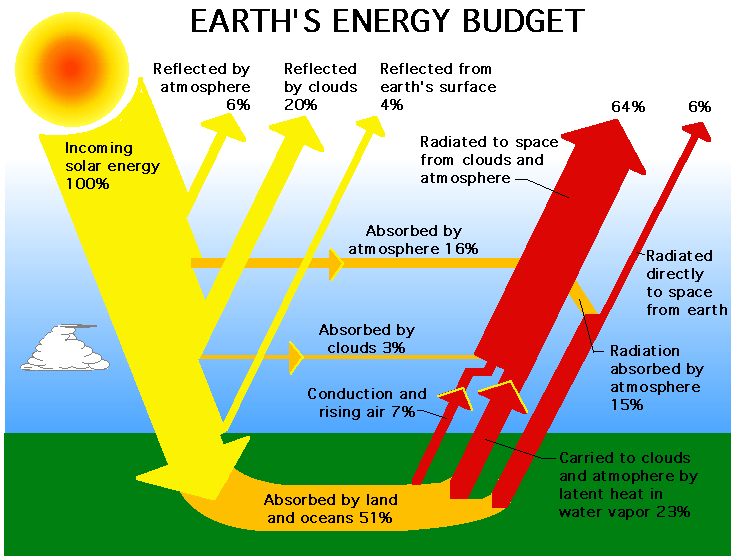
\includegraphics[width=\linewidth]{images/earth-system/earth-rad-budget-nasa-erbe.png}
\caption{caption}
\label{fig:earthbudget}
\end{figure}

Light enters the atmosphere, where some is absorbed and some is reflected. Light interacts in different ways with land, oceans, and vegetation, which is beyond the scope of our project. The ``quality'' of light changes through these processes. 

\subsection{The Spectrum of Light Entering and Exiting the Earth's Surface}

As the sun's electromagnetic radiation interacts with the Earth's Atmosphere, certain wavelengths are absorbed and filtered out (Figure~ \ref{fig:em-entering}).

\begin{figure}
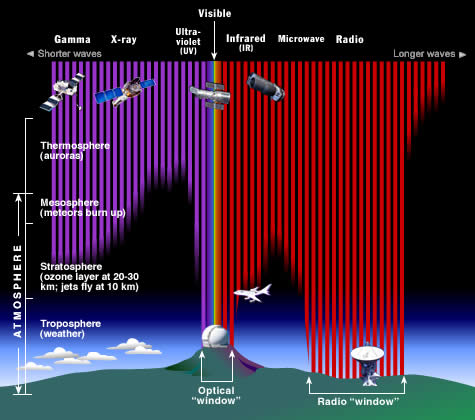
\includegraphics[width=\linewidth]{images/earth-system/em-radiation-atmosph-depth-stsci.jpg}
\caption{Various wavelengths of solar electromagnetic radiation penetrate Earth's atmosphere to various depths. Fortunately for us, all of the high energy X-rays and most UV is filtered out long before it reaches the ground. Much of the infrared radiation is also absorbed by our atmosphere far above our heads. Most radio waves do make it to the ground, along with a narrow `window' of IR, UV, and visible light frequencies. Source: STCI/JHU/NASA.}
\label{fig:em-entering}
\end{figure}

\subsection{The Atmosphere and Greenhouse Effect}



\section{Carbon Biogeochemistry}

\subsection{Long and Short Time Scales}

The carbon cycle processes occur at wide range of temporal scales from hundreds of millions of years to seasons of the year. These have been referred to as long and short carbon cycles. However, for our purposes, I will call them ``geologic carbon'' and ''biosphere carbon'' processes. 

\subsection{Rock Cycle and Geologic Carbon}

The carbon cycle describes changes in the fluxes and reservoirs of carbon in the Earth system. On very long time-scales, millions of years, the primary reservoirs of carbon are the atmosphere, ocean, and rocks (limestone). Carbon moves between these reservoirs through volcanic outgassing, silicate weathering, and limestone sedimentation. The carbon cycle is linked to Earth's energy balance through atmospheric carbon in the form of \carbondioxide, a greenhouse gas.

\subsubsection{Mountains and Erosion}

\ref{fig:carbonpools}

\begin{figure}
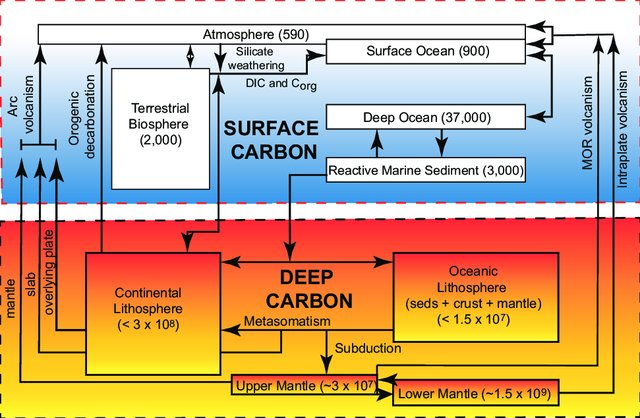
\includegraphics[width=\linewidth]{images/earth-system/Carbon-reservoirs-and-cycles-in-the-Earth.jpg}
\caption{Carbon reservoirs and cycles in the Earth. The figure shows short-and long-term cycles; biosphere and geologic carbon reservoirs and fluxes, and the relative sizes and residence times (y axis) of respective carbon. Numbers in brackets refer to the total mass of carbon in a given reservoir, in Pg C (1Pg C = 10$^{15}$ g carbon). All reservoirs are pre-industrial. Abbreviations: C org = organic carbon; DIC = dissolved inorganic carbon; MOR = mid ocean ridge; seds = sedimentary rocks. Adapted from Lee et al. (2019 And references therein).}
\label{fig:carbonpools}
\end{figure}

\subsubsection{Subduction Burial and Carbon Recycling}

Figure~\ref{fig:longtermcarbon}

\begin{figure}
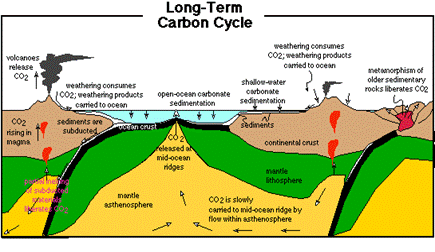
\includegraphics[width=\linewidth]{images/earth-system/long-term-carbon.png}
\caption{Schematic of the long-term carbon cycle (from Bice, 2001)}
\label{longtermcarbon}
\end{figure}

\subsection{Photosynthesis, Respiration, and Biosphere Carbon}

\subsubsection{Soil Respiration and the Soil Profile}

Carbon in soils is respired -- but different pools might have different rates of respiration. Sometimes these pools are distinquished as an active soil organic carbon pool and slow soil organic carbon pool. Although the reference of ``slow'' causes confusion with long-term, geologic carbon, but soil organic carbon remains a component of what we are refering to as biosphere carbon. 

The surface of the soil tends to have more SOC and microbes that can use that carbon for respiration. Lower down in the soil profile, we tend to see lower amounts of SOC and lower microbial biomass (Figure~\ref{fig:soilcarbon}. In addition, soils in the lower part of the profile tend to have more aggregation that protects SOC from microbial attack, thus a key area that soil carbon can seqeustor carbon. 

In addition to these microbial biomass and aggregate patterns, the microbes aree more senstive to temperature changes near the surface as measured by Q10 -- the rate of biochemical processes with a 10 degree C increase in temperature. Thus, soil processes, such as respiration, is likely to increase more near the surface with global warming that the lower part of the soil profile.  

\begin{figure}
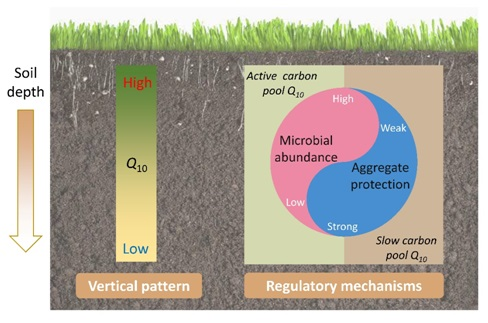
\includegraphics[width=\linewidth]{images/earth-system/Q10-SOC-Regulation.jpg}
\caption{Regulatory Mechanisms of the Temperature Sensitivity of Soil Organic Matter Decomposition in Alpine Grasslands (Source: \citet{Qineaau1218, CAS2021researchers}).}
\label{fig:Q10-SOC}
\end{figure}


\section{Fossil Fuels and Carbon Dioxide Trends}\label{sec:fossilfuels}

As part if the industrial revolution, our energy sources have put more \carbondioxide from the biosphere (soils and forests) and geologic carbon (coal, petroleum). 

\subsection{The Signal of Geologic and Biosphere Carbon in Atmosphere}

The combined contribution from geologic and biosphere carbon in the atmosphere is clearly documented from numerous sources. First, look at data collected at the Mauna Loa where \carbondioxide measurements have been taken continuously since the late 1950s. 

Figure~\ref{fig:maunaloa2}

\begin{figure}
\begin{knitrout}
\definecolor{shadecolor}{rgb}{0.969, 0.969, 0.969}\color{fgcolor}\begin{kframe}


{\ttfamily\noindent\bfseries\color{errorcolor}{\#\# Error in ggplot(train.data, aes(decimal.date, average)): object 'train.data' not found}}\end{kframe}
\end{knitrout}
\caption{Carbon Dioxide Measure on Mauna Loa, HI}
\label{fig:maunaloa2}
\end{figure}






\chapter{Monsoons and East Asia Climates}

\section{Temperature Gradients and Latitude}





\chapter{Critical Zone}\label{ch:critical-zone}

\chapterauthor{Marc Los Huertos}\footnote{The chapter was first drafted by Marc Los Huertos (2021). The author recieved valuable feedback from X, and Y and Z to improve the chapter.}

\section{What is the Critical Zone}

The crticical zone refers the the portion of the Earth's skin where the zone where rock meets life. The Critical Zone supports all terrestrial life.

The critical zone includes the following:

\begin{itemize}
  \item A permeable layer from the tops of the trees to the bottom of the groundwater;
  \item An environment where rock, soil, water, air, and living organisms interact and shape the Earth's surface;
  \item Water and atmospheric gases move through the porous Critical Zone, and living systems thrive in its surface and subsurface environments, shaped over time by biota, geology, and climate.
\end{itemize}

All this activity transforms rock and biomass into the central component of the Critical Zone - soil; it also creates one of the most heterogenous and complex regions on Earth.

Its complex interactions regulate the natural habitat and determine the availability of life-sustaining resources, such as food production and water quality.

These are but two of the many benefits or services provided by the Critical Zone. Such `Critical-Zone Services' expand upon the benefits provided by ecosystems to also include the coupled hydrologic, geochemical, and geomorphic processes that underpin those ecosystems.

\begin{figure}
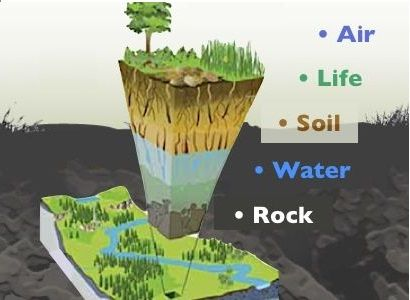
\includegraphics[width=\textwidth]{images/critical-zone/criticalzone.jpg}
\caption{The Critical Zone is an interdisciplinary field of research exploring the interactions among the land surface, vegetation, and water bodies, and extends through the pedosphere, unsaturated vadose zone, and saturated groundwater zone. Critical Zone science is the integration of Earth surface processes (such as landscape evolution, weathering, hydrology, geochemistry, and ecology) at multiple spatial and temporal scales and across anthropogenic gradients. These processes impact mass and energy exchange necessary for biomass productivity, chemical cycling, and water storage.}
\label{fig:criticalzone}
\end{figure}

\subsection{What are the environmental implications of the Critical Zone?}

The critical zone as a concept and as a material space pushes us to think of the porousity of the Earth's surface --- the gas and fluid flows through rocks, soils, and plants. We can begin to appreciate the complexity of the transport and fate of chemical pollutants as they enter the soil and become part of the vadose zone and perhaps the ground water table -- moving with water and diffusing through the water, simultaneously.

\section{Hydrologic Aspects}

\subsection{The Vadose Zone}

Jeji is a volcanic island is located some XX km south of the Korean Penisula. Water runs off the steep slopes quickly and water supplies are limited on the island. To adddress this...\citet{lee2017fifty}.

\begin{figure}
\includegraphics[width=\linewidth]{images/critical-zone/Lee-Vadose.png}
\caption{... (Source: \citep{lee2017fifty}).}
\label{fig:vadose2}
\end{figure}



\chapter{Land Use in East Asia}

chapterauthor{Samantha Beaton}

What is Land Use Change?

What Factors Drive Land Use Change?

How Land Use Change is Measured and Quantified

Integration of sociology

with data science: spatial data compiled from aerial photos, Landsat satellite images, topographic maps, GPS data, etc.

Requires classification and division of land-space types

Ecological Effects of Land Use Change on Soil, Air, and Water

\section{Impacts on Soil}

Deforestation and soil degradation

lack of stability (erosion) and loss of carbon sequestration potential

Forests


coupled with monoculture agriculture

Example Case Study: representative of monoculture agriculture-rice paddies in SE Asia (potentially\ldots)


Impacts on Local Watersheds

hydrology 

infiltration/pollution, groundwater recharge, flow of river basins, runoff

Higher risk of flooding and droughts

\section{Conclusion \& Prospect of Sustainable Urbanization/Land Use Change}


\chapter{Nuclear Power and Nuclear Waste}

\section{Current and Future Energy Needs}



\chapter{Air Pollution \& Social Justice in Hong Kong}

\chapterauthor{Neenah Vittum}

\section{Science of Air Pollution}

\subsection{Overview of the layers of the atmosphere/atmospheric gases}

What part of the atmosphere does air pollution affect?

What is air pollution?

Overview of different types of air pollution

\section{Major Sources → Use as geographical overview}

\subsection{General common sources of air pollution all over the world}

\subsection{East Asian countries/communities and their prominent air pollution sources}

Shipping

Traffic Emissions

Commercial and otherwise

Coal

Urban Development

Manufacturing

Other

The transboundary issue and its implications in regulation and politics

Impacts

Human health

Environmental Health

Greenhouse gas emissions and global warming

Both

Visibility

Environmental Justice

Case Study: Hong Kong

The Intersection of Air Pollution and Other Environmental Issues

Many environmental issues are interconnected

Air pollution and deforestation

Air pollution and urbanization/industrialization

Other Issues (To Explore)

Goals/Other Ideas/Questions

Ground information in geography and relevant examples

Incorporate stories and person accounts

slow violence → environmental justice issues

Maybe activist or someone who has suffered the issues firsthand

Draw people into the empathy

Use stories and descriptions to describe places

What is the best way to section the chapter?


\chapter{Flood Pulse System in East Asia}

\chapterauthor{Kristin Gabriel}

\section{Introduction}

What is the flood pulse system?

Seasonality

Ecosystem Services

Fish stocks

Flooded forests

How the flood pulse system influences the Tonle Sap Ecosystem

Timing of Flood Pulse

Magnitude of Flood Pulse

Duration of Flood Pulse

Influence of flood pulse system on people and their livelihoods

Fisheries

Immigration and emigration

Human Impacts on the flood pulse system

Climate change

Dam development

Case Study: Cambodia and the Tonle Sap


\chapter{Hydroelectric Dams in East Asia}

\section{Introduction}
    There exist over 48,000 hydroelectric dams worldwide (WWF Global, 2015) and have caused the forced displacement of between 40 and 80 million peopled (Hai, 2016). Hydroelectric dams account for 19\% of the world's electricity needs, in and some countries such as Vietnam, hydropower can cover up to 37\% of the country’s energy production. 
    
  One of the largest ironies of hydroelectricity is the benefactors and recipients of the produced energy. This is a process termed water grabbing. In most cases (specifically with mega dam construction), the produced electricity is either exported to nearby urban cities, or, in the case of regions like Laos, the energy is often exported to different countries altogether. This is in part due to the funders of dams and who facilitates construction. According to the BBC, Prior to the late 1900s (1940 to roughly 1970-1990), dam construction was funded by the World Bank (BBC).
  
  The World Bank began funding projects such as The Three Gorges Dam (one of the largest and most notorious hydroelectric dams) as well as the Sardar Sarovar Dam in India, the Chonoy in Guatemala, and the Itaparica hydropower project in Brazil as well as countless others. Beginning in the 1970s, criticism arose about the lack of social protection policies for the local and Indigenous communities that dam construction was impacting. Action was called to both assess, and end the harm caused by the World Bank so the World Commission on Dams was released, outlining the human rights abuses by the World Bank and they withdrew official funding from hydropower projects in the 1990s. Despite this, other corporations have filled the gap in funding, namely actors based in China such as the China Three Gorges Corporation and Sinohydro (Cooke, Nordensvard, Saat, Urban, and Siciliano). 
  
  Since the 1990s, there has been a surge in the amount of dams constructed in East Asia specifically, with over 10,000 of them (approximately 28\% of all worldwide dam construction) in Asia. Even within that disproportionate 28\%, a large number of dams lie in Laos which has been devastated by Chinese foreign investment and funders. Many even refer to Laos as the “Battery of [Southeast]Asia.” In cases of water grabbing in hydropower in Laos, energy is exported to other countries or urban cities and the Indigenous or local groups who were impacted by dam development are not granted access to the benefits of the dams that uprooted their lives. Many of these corporate projects have failed international guidelines on human rights and Indigenous rights, as well as ecological harms (which are often tied to subsistence and cultural reciprocity).  
  In many cases, the current social protection policies that do exist are lacking and can lead to justification for displacement. For example, relocation schemes enable hydropower companies to write off the harm they are causing to communities under the guise of some form of [insufficient] reparation. Furthermore, most relocation schemes force Indigenous communities into unideal cramped living conditions with poor infrastructure, sanitation, education, and without the ability to live with traditional modes of livelihood including but not limited to subsistence/agriculture, as well as cultural aspects of tradition such as crafts, styles, and familial structure. This, paired with the fact that in most cases of water grabbing in hydropower construction, the Indigenous communities displaced are moved into or not given access to the electricity their lives were destroyed to create. Instead, many Indigenous groups must find their own way to pay for or generate electricity should they desire it in their community.  



\section{Dam Function}
  Hydroelectric dams hold water in artificially created bodies of water, or reservoirs. To generate electricity, water is released through a turbine which spins a metal shaft (propeller) within the turbine to convert the energy of the flowing water into energy from movement, or mechanical energy (USGS). Because energy cannot be created or destroyed, the hydroelectric dams convert one form of energy (in this case the energy of the moving water), into another (watts to be distributed to a larger electrical grid for purposes such as energy for a household’s lighting) (U.S. Department of the Interior). This type of turbine that turns moving water’s energy into electricity is known as a hydraulic turbine.

\subsection{Hydroelectric Generators}
  Hydroelectric generators are based on the ideas of Michael Faraday who found that when a magnet moves past materials that allow electricity to flow easily, conductors, the magnet causes electricity to flow through the conductor. When direct currents of electricity are circulated through loops of wire around magnetic steel (electromagnets), poles of electromagnetivity are created (field poles). The field poles are put on the outside of the rotor which is attached to the turbine shaft.When the turned rotates, the field poles move past the conductors and electricity flows, causing an electromotive force, voltage, to develop. 
  
\subsection{Energy}
\subsubsection{Kinetic Energy}
  The size of reservoirs for hydroelectric dams can impact the amount of energy the dam can produce because of the pressure which impacts energy of motion, or kinetic energy. It is the amount of energy from the movement of the water which can be modeled with the equation. 
\begin{equation}
KE = 0.5mv%^2%
\end{equation}
In this equation, m is the mass of the object and v is the speed. This is important for hydroelectric dams because turbines can be spun through how quickly or strongly water travels in what is termed water flow. The mass of water is 18.015 g/mol and the speed depends on multiple factors, including the amount of pressure in the dam. For example, when using a hose to clean dirt from a surface, when the hose is hardly turned on, the flow is weak and slow. The water flow will not clean the surface very well because of the low amounts of moving energy. A hose turned on to its highest setting has larger amounts of water moving through the same sized hose at faster rates. This means the hose would have high amounts of moving energy and clean the dirt more efficiently. 
The same applies to hydroelectric dams and how their turbines are propelled to convert the moving energy. The higher speed and pressure means more moving energy which impacts how efficient a dam will be based on size and height. When thinking about a dam with a small reservoir, the amount of water will not create a lot of pressure on the released water, meaning the moving energy is low and the dam will produce fewer amounts of energy. A large dam reservoir will have high amounts of pressure and thus a greater moving or kinetic energy. 

\subsubsection{Potential Energy}
Similarly, the height of a dam impacts its energy potential. The higher a dam is, the more the water “falls” and the higher the potential energy is. Potential energy can be viewed as the amount of energy an object has (or has stored) if moved out of its equilibrium position, so when there is a further height to fall from, the stored or potential energy of the water is greater. This potential energy based on height or gravity can be modeled with the equation
\begin{equation}
PE_{grav}=mass*g*height
\end{equation}
In this, the PE grav is the potential energy, m is the mass, g is the gravitational strength (this is generally based on planet in which it will remain constant at about 9.8N/kg on Earth), and h is the height. The mass of water is also consistent at about 18.015 grams/mol on Earth. With this in mind, the gravitational potential energy of water (as is the case of hydropower) is based on the variable of height. The higher the dam, the greater the height, and the greater the potential energy.

\subsubsection{Total Mechanical Energy}
There is also a type of energy that is the energy of an object as the result of motion. In essence, it is the stored potential energy and motion energy when moved out of its equilibrium. To model this for falling water (this means we are not calculating the bounce of the object in motion, only the gravitational energy, the equation is
\begin{equation}
TME=PE+KE
\end{equation}
In this, TME stands for the Total Mechanical energy, PE is the potential energy, and KE is the kinetic energy. This means that the most basic way to model the total mechanical energy, or total produced energy, of a hydroelectric dam is dependent primarily on two factors, height of the dam and size of the dam. This is part of the reason that mega dams are favored by development companies—they have larger reservoirs and greater heights which allows the dams to produce more electricity, and thus garner larger profits, even though mega dams require exponentially larger volumes and surface areas which requires more local communities to be uprooted and increased deforestation and other ecological consequences. 
  
  
\subsection{Megawatts and Electricity Usage}

   Hydroelectric Dams produce an average of 42 billion kWh (kilowatt-hour) per year. This is enough energy to meet the needs of a developed residential area of about a million people, or 72 million barrels of oil (USBR). To put this into other perspective of just one megawatt is enough energy to power about 10 cars, or 300 homes an hour. Furthermore, part of the reason hydroelectric dams is touted as so efficient is because unlike alternate sustainable energy sources such as solar or wind, hydropower can run at all hours of the day regardless of weather conditions (Clean Energy Authority). 

\section{Hazards and Flooding}

  Another threat posed by the Three Gorges Dam is the impact it has on natural disasters. Due to alterations in the Yangtze’s hydrological patterns, sedimentation and saltation of the basin is also altered. As populations were forced to move, many of them moved to areas downstream of the Yangtze river into areas that are now considered floodplains due to the altered hydrology (World Commission on Dams 2000). It was predicted that there would be increased flooding and landslides as a result of the dam construction that has since been confirmed in the 21st century. 
    
  There was a documented increase in landslides in the 1990s in the Three Gorges region following dam construction. Of the almost 6,000 kilometers of reservoir shoreline, 5\% of it was considered dangerous and at risk for landslides (Wu 2001). With forced relocation, many people moved into the high-risk shoreline areas, putting them at huge risk for landslides. The increased risk of the landslides is due to the changed siltation and sedimentation which have the potential for loose rocks and sediment (Liu 2004). 
  
  Another risk posed by dam construction includes flooding; the alteration of hydrological patterns in the region means that previous flood plains are no longer flooded, and new flood plains are established, sometimes in areas population with humans. Estimates from the Sino-German Center for Research Promotion has documented up to 3,000 people having been killed due to flooding in 1998 as a result of the changed to the Yangtze River Basin due to construction. There also exists the possibility for dam collapse should an earthquake occur, although flooding and landslides are more common (World Commission on Dams 2000). 


\section{Three Gorges Dam}

Construction of one of the biggest hydroelectric dams, the Three Gorges Dam in the Yichang Hubei Province in China began in 1994 with the aim to prevent flooding, generate electricity, and to allow ocean freighter ship to navigate inland from Shanghai along the Yangtze river basin (Jackson and Sleigh, 2000). The Dam is estimated to have production capacity of 18,600-22,800 Megawatts of hydro powered electricity which accounts for about 10\% of all of China’s energy production (Li 2007). 
By 2012, the dam’s 32 turbine generators were all operational (Britannica). The dam’s reservoir holds 5.85 trillion gallons of water and is estimated by the dam’s beneficiaries to eliminate flood related damage for up to a century to protect human development on the banks of a river, or a riparian ecosystem. The dam produces about 84.68 billion kWh of clean energy a year (Wang and Bryant). The water flow on the Yangtze has also deepened by the dam to allow ships to carry commercial goods to and from Shanghai to reduce shipping costs by 35-37\% and thus increase profits for large commercial enterprises (Wang and Bryant).
The number of people displaced and affected by Three Gorges Dam is highly controversial, with estimates below one million (from the Dam’s developers) to 10.2 million people in 1996 (Delin and Lijun), and estimates ranging up to 900 million people affected (not displaced) due to disruptions in watersheds upstream or downstream of the dam (Childs-Johnson and Shen 2000). The local region and population around the dam prior to construction was below the poverty line and reliant on agriculture with dense but patchily populated areas (Delin and Lijun, 2000). Literacy rates were lower than the national average and upon construction of the dam, new townships were created to house the local displaced populations, but many displaced people were forced into urban centers for which they were poorly equipped to find work given their reliance on subsistence farming previously (Cernea, 2003). 30,000 hectares of farmland that local populations once relied on were flooded and water borne illnesses such as schistosomiasis and other diseases such as tuberculosis and pneumonia become more common in relocation areas due to reduced access to sanitation (Jackson and Sleigh, 2000; Cernea, 2003). 
Furthermore, psychosocial impacts on the displaced populations were devastating. The complete forced shift away from traditional livelihoods as well as loss of cultural sites and disintegration of social support networks caused traumatic stress, stigmatization, depression, and inter-community violence as a result of the destruction (World Health Organization, 1999). The Yangtze (a watershed involved in the dam) is known as the “sorrow of China” due to the millions of lives the dam project has destroyed both through forced displacement, and even death due to natural disasters. (Sino-German Center for Research Promotion 2006).

\subsection{Displacement}
  One of the common costs of “development” is displacement of local and Indigenous populations—hydroelectric dams are no different. Due to the fact that flood plains are covered in water, the reservoirs themselves take up large amounts of space, and local hydrology is often drastically altered as a result of dam construction, forced displacement is a common result of dam building. Displaced has further implications for even more construction and development for the displaced populations—new infrastructure such as hospitals, schools, roads, water irrigation, and electricity needs to be set up for displaced populations. Unfortunately, new infrastructure for forcibly displaced peoples often is insufficient or inadequate to sustain populations. 
  
  One measurement of human well-being following construction of the Three Gorges Dam was done my Millennium Ecosystem Assessments (MA) in 2003 by the Millenium Ecosystem Assessment and World Resources Institute. They classify human well-being under five categories: “access to basic materials, freedom and choice, health, social relations and social capital, and security” (Millenium Ecosystem Assessment (MA) 2003, Table 1). Due to a number of factors, the MA assessment concluded that the Three Gorges Dam does not meet the requirements to be socially responsible and equitable. 

\subsection{Schistosomiasis}

Snail fever, or schistosomiasis is a disease from parasitic worms called schistosomes. Schistosomiasis causes abdominal pain, diarrhea, bloody stool, or blood in urine (CDC). Schistosomes typically live in freshwater snails which are vectors of the disease. The parasite comes out of the snail in freshwater and humans can become infected from skin contact with the contaminated freshwater (CDC). Snails infected with schistosomes live in freshwater dams such as the Three Gorges Dam (Liang 2002). 
Schistosomiasis is found only in certain areas, making it endemic, but along with the construction of hydroelectric dams, it is common that snails become vectors for the disease, and they bring Schistosomiasis from the endemic regions. The dams bring in larger quantities of snails every year, making the disease more common (Zhu). Due to displacement of local populations due to dam construction, this often means influxes of people from schistosomiasis endemic zones enter greater populated areas and this leads to an increase in infections.
One of the dams in East Asia that experiences cases of schistosomiasis is the Three Gorges Dam. There is a narrow reservoir attached to the dam that is 1084 km SQUARED which extends into the Jianhan Plain in the Hubei Province and the Chengdu Plains in the Sichuan province—both regions are endemic for schistosomiasis (Wang and Zheng 2003).
There are many cases of increased schistosomiasis because of dam construction throughout the globe such as Egypt, Senegal, and other continents such as South America. African snails for example, have thin and lightweight shells that make their dispersal throughout regions especially effective and dangerous (Li and Lin 1998). Following construction of the Diama dam in Senegal, a strain of infection from S. mansoni snails occurred due to the stabilized water levels. Inadequate health care services in the area of the Diama dam led to an outbreak infection everyone in the city of Richard-Toll (in the dam region) (Waldstein 1997). 
There do exist differences between the case of the Diama dam and that of the three Gorges Dam, including the type of snails in the region, despite this, the Diama dam should serve as a cautionary tale for large dam construction such as the Three Gorges Dam. Healthcare for displaced populations is limited and due to numerous factors, the Three Gorges dam construction poses increased risk for snail dispersal, breeding, and survival. The most common type of snails in East Asian regions such as the Three Gorges Dam is the O. Hupensis (Mao and Shao 2018) or S. japonicum snail (Jordan 1993). For the purposes of this case study of the Three Gorges Dam and schistosomiasis, the “snails” referred to are of the O. hupensis or S. Japonicum variety. 
The Center for Disease Control and Prevention (the CDC) observed that schistosomiasis cases occurred frequently in the Three Gorges area after the construction of the dam, with estimates of up to 100,000 cases of infection. If these cases return to their homes from hospitals, the presence of O. hubensis in the region could mean their co-existence can lead to increased numbers of infected snails, and later, increased cases in humans. In comparison to other areas of the world, proponents of the Three Gorges Dam argue that there is no correlation between cases of schistosomiasis and the dam, but as evidenced by Zhu and other authors, The Three Gorges Dam may make the region more susceptible to both O. hubensis (vectors for the disease), and thus increased cases among humans.


\subsubsection{Temperature}

  One factor that has the potential to draw snails to the region of the Three Gorges Dam is the ideal temperature for the snails. By using Geographic Information Systems, a study showed with a 95\% confidence interval that the compatible range for the snails was 0.9°-21.1° C. The Three Gorges region’s average temperature is 3.9-18.8° C which is not quite currently compatible with that of the snails. Despite this, because the dam has a greater heat capacity than naturally occurring bodies of water in the area, the average temperatures have the potential to increase in a range from 0.3-1.2° C depending on the season, making the climate changes more compatible with the snail’s ideal temperatures which may make the region around the dam increasingly ideal for their presence (Peng 2006). 

\subsubsection{Breeding Patterns and Resettlement}

  As displacement of millions occurred due to the construction of the dam, migrants resettle their homes often as close to their homes as possible away from the reservoir. This means that slopes or hilly areas near the dam are newly inhabited by farmers and the displaced populations, causing soil erosion in the farmed resettled regions, and it causes increased silt deposits in the Hubei region (recall this is a region endemic to the snails). This causes sedimentation and creation of marshlands in areas such as Hubei which are conducive to snail reproduction (Lai 2000).  

\subsubsection{Snail Movement}

  Snails are distributed or dispersed throughout regions in two ways—actively and passively (Wu 2005). An example of passive dispersal is snails attaching to ships that move to new areas. Active dispersal can look like snails moving across regions via water currents. Passive dispersal does not necessarily have a limit to potential distance traveled, but through active dispersal, a snail can travel distances of up to 168 kilometers (Zhu 2008). The closest endemic region to the dam itself is 299 kilometers and there have been documented cases of paper-making reeds that snails and snail eggs have lived on which carried the infected snails across large distances into paper factories in the region (Wei 2004). Documented cases such as these imply that the snails could have made their way to the dam from endemic regions through passive dispersal such as the paper-making reeds, or even soil brought into the region that contains snail eggs. Zhu suggests that as the Yangtze River facilitates more merchandise to be brought into the region, there is a greater chance of more infected snails to also enter through passive dispersal. 

\subsubsection{Health Infrastructure}

  One of the reasons the risk for Schistosomiasis remains high in the Three Gorges Region is because relocated populations are moved into crowded urban areas which make the possibility for outbreaks and spread of disease higher. Furthermore, there is insufficient infrastructure (I.e., Hospitals, clean water, or proper sanitation) to prevent, or treat the disease. Crowded living arrangements with multiple generations forced into crowded housing also does not aid either sanitation, or the prevention of the spread. For this reason, transmission of diseases such as Schistosomiasis is a threat and danger. Other diseases (water borne or otherwise) are also common, including but not limited to hepatitis, pneumonia, diarrhea, and a virus often spread through rodents—Hantavirus. 

\subsection{Eutrophication}

  One of the issues with the dam is altered hydrological flows and increased nutrient sedimentation and toxin buildup. The Three Gorges Reservoir is fed by the Yangtze River (among others). There have been shifts in both water flow, and water levels in the Yangtze as a result and it disrupts the aquatic life, including but not limited to the plankton and microbes of the river (Sekiguchi 2002). An excess of nutrients from runoff leading to dangerously low depleted oxygen levels in the water, a process called eutrophication, has occurred in the Yangtze and its tributaries and watersheds. Agricultural practices that were once not harmful are now causing the eutrophication due to the changed water levels and flows (Liu 2002). 

  Furthermore, industrialization in areas of the Yangtze River watershed has occurred, due in part because of extending urbanization from other areas, as well as urbanization of the displaced populations due to the dam construction. For this reason, the nutrient runoff and toxin runoff associated with industrialization and urbanization has worsened (Zheng 2008). Because of the excess of nutrients associated with eutrophication, there have been increased number of scum and deleterious (dangerous) toxins such as neurotoxins which are a threat to public health—this growth as a result of nutrient excess of nutrient loading is known as cyanobacterial algo blooms (Mei 2003). This buildup of toxins that effects the water quality is especially prevalent in the Three Gorges region because of the amount of subsistence farming that occurs. 
  
  Most of the local populations in the Three Gorges regions live rural agrarian lives based on subsistence. Populations along the Yangtze River that do rely on the subsistence farming are also hugely dependent on the river for a water source. As the water quality decreases with eutrophication and the buildup of toxins, the local populations that rely on the water and soil nearby are exposed to the toxins that are caused upstream due to industrialization. The water quality can impact crops and nutritional needs, but also daily life water usage such as washing and cleaning. One of the less deadly diseases is a dietary disease that can cause tooth decay and destruction due to excess fluoride in a water source—this is known as fluorosis and is common in subsistence populations who live near the Yangtze river (World Health Organization 1999).


\section{Social Systems and Infrastructure}
  As a result of millions of people being forcibly relocated, there exists the issue of where to relocate. Some populations move downstream or into regions nearby, maintaining some level of autonomy and subsistence that they had prior to their displacement. Despite having lost often culturally significant lands, this seems to be a better option for many than those who are forced into townships or urban areas such as Chongming—an island city at the mouth of the Yangtze in Shanghai that has been growing in population and size where many displaced populations from the Three Gorges Dam were relocated to. In these cases, the displaced populations are forced into areas with existing political institutions which causes social unrest, resentment, and discontent among populations who were once primarily autonomous. 
  
  Within these townships and urban centers, there often does not exist sufficient living space or housing, education, health care, sanitation, job opportunities, space for subsistence farming/traditional careers, and ironically, energy or electricity. With the loss of 30,000 ha of farming land and government policies to discourage subsistence farming in the region (known as “de-farming”), malnutrition has increased. Almost half of the resettled populations will not have access or resources to farm and provide subsistence for themselves, driving them away from agrarian jobs into industrial careers (Jim and Yang 2006). This can be detrimental to mental health and personal/individual agency when stripped of the ability to provide for oneself through traditional modes of subsistence (Jackson and Sleigh 2000). 
  
  The World Health Organizations reported that the psychosocial effects of the displacement have caused traumatic stress, mental health issues such as depression, and increased violence as a result of the aforementioned. Furthermore, social and cultural networks that were once in place in communities collapsed following displacement in many cases. Communities were split up or simply altered so significantly that the social support that was once available has disintegrated. This too causes mental illnesses such as depression. With a lack of health care system for both physical and mental needs, none of the mental health issues are addressed at a health care level. 

\subsection{Food Security}
  Furthermore, lack of availability of traditional food sources have led to inadequate diets that have documented cases of having caused chronic diseases and ailments (Millennium Ecosystem Assessment (MA) 2005). It would be naïve to group all populations impact by hydroelectric dam construction under the same universal or to assume they all rely on the same modes of livelihood, but a large majority of local or Indigenous populations in dam construction regions rely on agrarian lifestyles. Groups such as the community of Long Lawen and neighboring villages in Malaysian Borneo for example rely on agriculture, hunting, and fishing and this is the case with most other villages in numerous villages in East Asia near dams such as the Three Gorges or Bakun dams. For example, Laos or Lao PDR (known as the “Battery of Asia” because of the number of hydroelectric dams in the country), relies on agriculture for up to 80\% of employment and almost a quarter of the country lives at or below the international poverty line (MONROE 2016). 
  
  Using Laos again as an example, the threat to subsistence for forcibly displaced or impacted populations. Rural populations in Laos rely on fish for anywhere between 47-80\% of their protein intake in their daily diets, often supplemented by carbohydrates and fats from other sources including (though not limited to) crops from farming. This means that when displacement occurs, or when watersheds are altered (i.e., flooding to create reservoirs, eutrophication, or other alterations to water quality), so too is subsistence and traditional food sources are disrupted. This often leads to malnutrition and simply insufficient amounts of food. A case study that briefly illustrates this is that of the Ladakh people. Anthropologist and author Helena Norberg-Hodge did a study of the Indigenous Ladakh people and found that with the introduction of dam construction and western development, the Ladakhi’s shifted away from traditional subsistence (both forcibly and willingly). In her time with the Ladakh people, she noticed a shift in diet from the agrarian crops produced, to less nutritious options such as instant noodles which are increasingly popular as an affordable food source for Indigenous populations who no longer have access to farmland or fish. This leads to malnutrition as well as psychosocial impacts from a shift away from traditional nutritious food sources for Indigenous and displaced populations.

\subsection{Cultural Sites}
  Another issue that is posed by the displacement and forced relocation lies in the loss of cultural sites. Estimates of more than 140 villages were destroyed due the dam and it has been impossible to even count the number of cultural sites lost, as well as their value to communities (Childs-Johnson and Shen 2000). This loss of cultural sites such as traditional alters, ancestral lands, or other culturally significant landmarks, topographical features, homes, burial grounds, and other sites lost to the dam construction is incalculable. It is truly impossible to do an accurate cost benefit analysis when comparing the number of megawatts produced as opposed to the unquantifiable number of cultural sites lost and lives altered.
  
  Entire towns and temples have been flooded by singular dam development. The Three Gorges Dam for example submerged the White Crane Ridge—a hydrology inscription--, the original sites of the Zhangfei Temple—a temple that was removed by archeologists from its original location to prevent it from being completely submerged--, and Dachang—an ancient town that was submerged and had to be replicated/rebuilt downstream (Childs-Johnson and Shen).


\section{Vietnam and the Hoa Binh Dam}
  One of the country's most reliant on hydroelectric energy is Vietnam due to its Riparian ecosystem that makes it ideal for the dams. Between 1995 and 2009, 20 large scale hydropower dams with capacities of more than 100 Megawatts were constructed in Vietnam (Ty, and Westen, 2011). Most of the dams were built in areas populated by ethnic minorities with more than 144 dam investment projects in the Kon Tum and Dak Nong provinces (both rural areas populated with ethnic minorities) (Ngoc Lan, 2008). 
  
  Dak Nong for example is located in Vietnam in the central highlands in a mountainous region with generally nutrient rich soils due to high levels of basalt which makes it ideal for farming and many of the people in the Dak Nong province farm coffee, rubber, cashews, sugar cane, and pepper trees. Around 85\% of the population lives in rural areas and it is one of the poorest provinces in Vietnam. Furthermore, the Vietnamese government made it a priority to bring electricity to Indigenous and rural communities in 2004 to reach 100\% of households by 2020 but these goals were not met. Instead, rampant dam construction has occurred at the expense of the Indigenous populations the Vietnamese government tried [and failed] to bring electricity to and they instead ravaged local ecology in the name of progress and energy (RISIREA). 
  
  The dams in this area caused damage to forests and altered river streams and flow speeds, causing sedimentation and erosion which threatened the biodiversity of the rivers and surrounding areas. The 200-kilometer Hoa Binh Dam displaced 58,000 people, 79\% of whom belonged to ethnic minority groups including the Muong, Tay, Dao, Thai Trang and Thai Den (Nga Dao, 2010). The dam destroyed 20,800 hectares of farmland, crop fields, and forests which were crucial to traditional production and subsistence practices of the rural poor in the area (Yen, 2003). 
  
  The Muong people for example are the second largest ethnic minority in Vietnam and the largest ethnic minority in the Indochina region. They rely on agrarian farming with crops such as rice. They rely on local ecology for subsistence including crops, hunting, and raising animals. They also engage with outside economies to some extent as they gather wood and cinnamon for trade. The destroyed farmland and crop fields were incredibly destructive for the Muong living in the region impacted by the Hoa Binh dam as it stripped necessary farmland and forests necessary for subsistence as well as products to trade (Britannica). 
  
  Of the 58,000 people displaced by the dam and surrounding destruction to the ecosystem, clean water, education, healthcare, and other basic human needs were unavailable. Up to 34\% of the displaced population did not have access to clean water, and ironically, 20\% of them did not have access to electricity (regardless of the fact that their displacement stemmed from exploitation of their lands to produce electricity for the national grid which they did not have access to). In 2009, poverty rates of the displaced population were 59-60\% compared to the national rate of 14\%. Primary school completion was also almost 10\% lower than the national rate. The Hoa Binh hydropower project demonstrates the lack of comprehensive Environmental Impact Assessments (EIA) and sustainable relocation plans—allowing for the valuation of profit over human life (Hai 2016). 

\section{Long Lawen and Long Liam}
  Another case study that is important for understanding Indigenous sovereignty alongside the issue of hydroelectric dams is that of Malaysian Borneo, and more specifically, the villages of Long Lawen and Long Liam. Both villages are case studies in which the people protested or refused resettlement and dam construction and they found energy alternatives. This is not to say hydropower development has a “happy ending” but Long Lawen and Long Liam are arguably more optimistic case studies for the autonomy and advocacy in Indigenous communities.  

  To begin, Long Lawen set some model of an example for what is called micro hydro projects as termed by Headman Gara Jalong of the village. He has been fighting for many years to protect Long Lawen, often at the cost of imprisonment. In the 1990s, the Bakun company tried to forcibly remove the community of Long Lawen to build a mega-hydropower dam called the Bakun Dam. It is one of the largest dams in Southeast Asia to this day in the rainforest in the Belago District in East Malaysia in Sarawak on the Balui river. The village of Long Lawen lives in this area and their original location was in the way of dam construction. The dam is 14,170 kilometers squared (which for reference, is the size of the entire country of Singapore—this is an extremely large dam). It occupies 12\% of Sarawak and its main funder is a Chinese company. During construction of the dam, the company Bakun was practically uninvolved with the relocation scheme which they left to the local government in Borneo. This relocation scheme required the removal of the Long Lawen village and was intended to remove them to a government-controlled site, stripping them of their cultural autonomy and land.  

  Gara Jalong, as well the community members refused the government’s resettlement plan and the community moved independently in a safe area above the dam construction. While an imperfect solution (which already is flawed as Long Lawen should not have been presented with the requirement to move at all), this did allow Long Lawen to remain somewhat autonomous and independent as opposed to moving into the government-controlled resettlement location.  

  Long Lawen still remains in the rainforest in longhouses with connected apartments for the community members which is the traditional style of residency, and it is not uncommon for the older generation to maintain many of the traditional practices such as stretched long ears, as well as traditional modes of livelihood such as creating forest products and hunting and fishing. It is also common for many members of the younger generation to prefer western fashion or living in a transition very similar to the Ladakh people that we read about in Ancient Futures. Many of them have moved out of Long Lawen but they still visit annually.  

  In 2000, the Malaysian Senator Banie Lasimbang helped Long-Lawen build a micro-hydro turbine. The science of these micro-dams remains like that of mega-dams (a turbine utilizes gravity to turn and generate electricity), but a key difference is that this micro-hydro power installation was built by, approved by, and desired by the community of Long-Lawen. 

  Through Senator Banie’s help, Gara Jalong and the community were able to construct a dam that did not displace them or alter their watershed to detrimental effects. One of the largest ironies of hydroelectric dams as mega projects by outside contractors is that the local and Indigenous communities they displace almost never receive the benefits of the generated electricity. This is the case with Long Lawen which made the micro-dam so appealing to bring “cleaner” and arguably better electricity to the village as it was advocated for by the community members themselves.  

  There are of course limitations to the micro-hydroelectric dams, including but not limited to the amount of energy they produce. For example, during the winter holidays, younger community members and extended family members of the Long Lawen community return home and during this time, the 4-6 kilowatts a day produced by the dam is insufficient for the village. The micro dam was supposed to produce up to 12 kilowatts of electricity a day, but the actual numbers have fallen quite short of those estimates.  

  Despite the lower energy production than anticipated, the micro dams have been replicated in almost a dozen other villages in the region including Long Liam who also built a micro dam using Long Lawen as an example. The village of Long Liam also ran into issues with their dam, including technical problems. A feature of hydroelectric dams is a penstock which channels the water towards the turbine, but in the case of Long Liam’s micro dam, the pathway towards the penstock isn't a straight path which complicated the efficiency of the energy production. While this is technically fixable, it would require manual labor and be difficult to fix without some level of alteration to the ecosystem (notably though, this alteration would be considerably less than any destruction caused by mega dams, and it would be facilitated by the community members).  

  This is not an argument in favor of the mega dams, nor for energy sources such as fossil fuel, just an acknowledgement of the inadequacy of micro dams as a sole energy source for a village. Mega dams are so harmful in both the social aspect, as well as the ecological aspect that micro dams may in fact be a potential alternative to the alternative energy source of mega dams. 

  Author of the book Ancient Futures, Helena Norberg-Hodge argues for a transition from globalization and globally based economies/development (such as mega dams), towards localization of agriculture, as well as energy production. She advocates for small-scale energy development projects such as micro dams, but explains that “when it comes to small-scale projects that truly promote self-reliance, such as village-scale hydroelectric installations or solar ovens and water heaters for the household, the question is immediately asked: ‘Can the people pay?’ Nuclear reactors and big dams are heavily subsidized, while small scale-technologies based on renewable energy receive no significant support from any major aid agencies” (Norberg-Hodge 146-147). While I believe there is a very fine line to balance between imposition of western technology and aid, I believe that should Indigenous communities or villages desire such village-scale installations of hydroelectric dams (or other energy sources), it is the obligation of global aid organizations to subsidize, or even fully fund such projects. I believe this is a place we can begin to remedy some of the harm we have caused given there is desire for it from the community for such small-scale development (although again, this decision would need to be make through Indigenous sovereignty at the community decision making level)  

  An important part of this desire can be explained by Author John Bodley’s proposal for cultural autonomy for Indigenous nations. He says that its purpose is “establishing the Indigenous peoples’ right to self-determination and ‘helping to secure the future of Indigenous cultures in concurrence with their own efforts and desires... 1. to focus international attention on the contemporary situation of Indigenous peoples 2. To pressure governments to respect the internationally recognized rights of Indigenous peoples 3. to provide financial assistance to Indigenous peoples in support of their self-determination struggle (280) which would “permit tribal peoples to choose the degree of isolation they want to maintain (295). I think these ideas of cultural autonomy for Indigenous community is key in the discussion of both mega and micro hydroelectric dams. Part of the reason most hydropower development so radically violates Indigenous rights is because it ignores land rights and human rights as well as the desires of the Indigenous communities and their right to make decisions for themselves. If village-scale hydropower is an avenue to further explore in terms of electricity generation, it must comply with ideas of cultural autonomy. In other words, any development, even at the micro scale, must permit Indigenous groups to determine the level of involvement and development they would want in their villages.  

  The alternative energy source of mega dams is far from “clean” or “sustainable” both from an ecological standpoint, as well as from a humanitarian point of view. The water-grabbing that occurs in the mega dam development results in clear winners and losers as big construction companies profit off the ecological degradation and human impact of the dams. The displaced populations face loss of culturally important homelands, as well as threats to social systems and modes of livelihood that are clear violations of cultural autonomy and Indigenous rights. We must halt mega dam construction for good and at least attempt to give back autonomy and agency to the Indigenous groups so deeply impacted. In the face of the Climate Crisis,a departure from this avenue of “cleaner” energy production must not occur, but it is key to ensure hydro power projects are smaller, do not cause displacement, and are done at the behest of the local populations they will impact.  

\section{Conclusion}



\chapter{Climate Change and Food Security in Myanmar}



\section{Climate Change, Climate Change Response in Myanmar}


General history of rice production and food demand in Myanmar. 

Impact on credit policy on rice 

Impact of infrastructure development on rice production

Study of the constraints of rice production in Myanmar

The effect of a command economy on food production in Myanmar 

Overall review on demand for food in Myanmar 

Possible implementation of SRI (systemic rice intensification) in order to increase rice yields in Myanmar

Transition from talking about rice production

sea-level rise

subsidence

coastal erosion

coastal flooding

Impact of climate change on rice production in Southeast Asia

Monsoon Season effect on Ayeyarwady River Badin

Sea Level Rise 

Sea level rise effect on global markets/rice production


Subsidence

Subsidence in Yangon, Myanmar

interview segments/personal experiences of rice farmers


Roles of the Burmese government

\section{Conclusion}

Reminders/Areas of Focus




\chapter{Disasters, Typhoons and Phillipines}

\chapterauthor{Ian Horsburgh}

\section{What are Typhoons?}



\chapter{Climate Infrastructure in Vietnam}

\section{Introductory}

How climate change will impact Vietnam

Flooding (especially coastal urban areas)

Sea Level Rise

Land Erosion

Health outcomes

Current Adaptation Plans

Strengthen existing barriers and infrastructure

Adapt cities expecting sea level rise

Withdraw from the coastlines in areas that are well below sea level

What's Needed for the Future

Stronger healthcare system

Support for farmers and agricultural workers

Support for rural population near Mekong and Red river deltas

\section{Conclusion}

Implications for other places in the region


\chapter{Waste Management for a Circular Economy}

\section{Life-Cycle}

\subsection{Collection}

\subsection{Transport}

Treatment

Disposal

Sectors:

Industrial

Household

Biological 

Types of Waste:

Solid:

Liquid

Gaseous waste

\section{Biomimicry}

\subsection{Circularity}

Examples in Nature

Education:

Teach people to be mindful and live sustainably

Social PsychologyProblems and New Approaches: 

Sustainability

Incineration \& Dumping

Recycle \& Reuse

Resource Recovery


\chapter{Plastic and Packaging in Japan}

\section{Introductiona and Goals?}

Plan: Use Japan's unique plastic packaging as a lens to view plastic waste management. I can bring in benefits of their plastic use, like cultural significance of beautiful wrapping and food safety, and then discuss plastic pollution as a larger issue in East Asia, bringing in examples of blame placing, and of course discussing potential solutions on both international and local scales. 

\section{Plastic Pollution and Waste Management in East Asia} 

\subsection{Statistics/comparisons}

graphs and images will help with perspective

\subsection{History of plastic waste issues in East Asia}

\subsubsection{Are specific companies/industries responsible responsible}

what kinds of plastic waste are there (sector break down)? 

\subsubsection{Where in the world did the ubiquitous usage of single use plastics come from?}

General blame placing/biases/rhetorical 

examples of discourse around plastic waste in East Asia. Why does any of this matter(needs its own section)?

Plastic waste trade? 

\url{https://link.springer.com/article/10.1007%2Fs10163-004-0115-0}

\url{https://www.sciencedirect.com/science/article/abs/pii/S0956053X20305602}

Blame placing through both rhetoric and scientific studies

(this source is a very data based study that concluded that the vast majority of plastic pollution comes from a few sources in Asia/Africa... I want to explore what they might not have taken into account when collecting data)

\url{https://science.sciencemag.org/content/347/6223/768}

\url{https://pubs.acs.org/doi/10.1021/acs.est.7b02368}

\url{https://www.dw.com/en/whose-fault-is-plastic-waste-in-the-ocean/a-49745660} (found the two above studies through this article)

Japan Specific (I need to break these into hierarchies of significance), some sections, the first  few will be more data based, the second half will be more rooted in sociological primary sources.

Waste management issue overview

Sector Break Down/ responsible parties in Japan

Impacts of plastic pollution on different groups within Japan

Cultural significance of wrapping

Food safety

Gov action/recycling/current efforts

Activism

Potential solutions moving forward rooted in current activist efforts/respect to culture

\url{https://www.pnas.org/content/117/33/19844.short}

\url{https://www.jstor.org/stable/432317?seq=1}

\url{https://onlinelibrary.wiley.com/doi/abs/10.1002/1099-1522(200003/04)13:2%3C45::AID-PTS496%3E3.0.CO;2-%23}






\backmatter

\part{Backmatter}

The back matter often includes one or more of an index, an afterword, acknowledgments, a bibliography, a colophon, or any other similar item. In the back matter, chapters do not produce a chapter number, but they are entered in the table of contents. If you are not using anything in the back matter, you can delete the back matter TeX field and everything that follows it.

\printglossary

\renewcommand\bibname{References}
\setlength{\bibsep}{2\baselineskip}
\setlength\bibindent{.5in}
\bibliographystyle{plainnat}
\bibliography{References}

\end{document}
